\documentclass[aspectratio=169]{beamer}
\usetheme{focus}

%\usepackage{beamerthemesplit}
%\beamertemplatenavigationsymbolsempty
\usepackage{amsmath}
\usepackage{amsthm}
\usepackage{amssymb}
\usepackage{latexsym}
\usepackage{graphicx}
\usepackage{fancybox}
\usepackage{dsfont}
\usepackage{multirow} 
\usepackage{multicol}
\usepackage{booktabs} 
\usepackage{dcolumn}
\usepackage{soul}
\usepackage[cache=false]{minted}
\usepackage{MnSymbol}
\usepackage{stmaryrd}


\DeclareMathOperator*{\argmax}{arg\,max}
\DeclareMathOperator*{\argmin}{arg\,min}

\newcommand{\X}{\mathtt{X}}
\newcommand{\Y}{\mathtt{Y}}

%\newcommand{\R}{\mathbb{R}}
%\newcommand{\E}{\mathbb{E}}
%\newcommand{\V}{\mathbb{V}}
\newcommand{\p}{\mathbb{P}}
\newcommand*\df{\mathop{}\!\mathrm{d}}
\newcommand{\del}{\partial}


% imports
\usepackage{xargs}
\usepackage{xpatch}
\usepackage{etoolbox}
\usepackage{pdflscape}
\usepackage{booktabs}
\usepackage{threeparttable}
\usepackage[skip=0.2\baselineskip]{caption}

% command for inputting raw latex
\makeatletter
\newcommand\primitiveinput[1]{\@@input #1 }
\makeatother

% common table command
\newcommandx{\tablecontent}[4]{
    \begin{threeparttable}[!ht]
        \centering
        \caption{#3}
        \vspace{-1em}
        \footnotesize
        \begin{tabular}{#1}
            \primitiveinput{../tables/#2.tex}
        \end{tabular}
        \vspace{-0.2em}
        \begin{tablenotes}[flushleft]
            #4
        \end{tablenotes}
    \end{threeparttable}
}




% \usepackage{slashbox}
\title{Lecture 2: Basics of Panel Data}
\author{Chris Conlon }
\institute{NYU Stern }


\newcommand{\norm}[1]{\left\lVert#1\right\rVert}
\newcommand{\R}{\mathbb{R}}
\newcommand{\E}{\mathbb{E}}
\newcommand{\V}{\mathbb{V}}
\newcommand{\ol}{\overline}
%\newcommand{\ul}{\underline}
\newcommand{\pp}{{\prime \prime}}
\newcommand{\ppp}{{\prime \prime \prime}}
\newcommand{\policy}{\gamma}


\newcommand{\fp}{\frame[plain]}

\date{\today}

\begin{document}
\maketitle



\section{Advanced Linear Models}

\begin{frame}{Hierarchical Linear Models}
An Example
\begin{align*}
Y_{it} &= X_{it}'\beta_i + \varepsilon_{it}\\
\varepsilon_{it} | X_{it} &\sim N(0,\sigma^2)
\end{align*}

Two Possibilities:
\begin{align*}
\left( \begin{array} { c } { \beta _ { 1 } } \\ { \vdots } \\ { \beta _ { N } } \end{array} \right) \sim \mathcal { N } \left( \left( \begin{array} { c } { 0 } \\ { \vdots } \\ { 0 } \end{array} \right) , \tau ^ { 2 } \cdot 
\left( \begin{array} { c c c } { \mathcal { I } _ { \mathcal { K } } } & { \ldots } & { 0 } \\ { \vdots } & { \ddots } & { \vdots } \\ { 0 } & { \cdots } & { I _ { \mathcal { K } } } \end{array} 
\right) 
\right)
\end{align*}


\begin{align*}
\left( \begin{array} { c } { \beta _ { 1 } } \\ { \vdots } \\ { \beta _ { N } } \end{array} \right) \sim \mathcal { N } \left( \left( \begin{array} { c } { 0 } \\ { \vdots } \\ { 0 } \end{array} \right) , \tau ^ { 2 } \cdot 
\left( \begin{array} { c c c } { \mathcal { I } _ { \mathcal { K } } } & { \ldots } & { \rho \cdot \mathcal { I } _ { \mathcal { K } } } \\ { \vdots } & { \ddots } & { \vdots } \\ { \rho \cdot \mathcal { I } _ { \mathcal { K } } } & { \ldots } & { \mathcal { I } _ { \kappa } } \end{array} 
\right) \right)
\end{align*}



\end{frame}

\begin{frame}[fragile]{Packages for Today}
Let's load some packages so that I can make some better looking plots:\\
\begin{minted}{R}
#always
library(tidyverse)
# for SE's
library(estimatr)
library(broom)
# for Panel
library(lfe)
library(plm)
\end{minted}
\end{frame}




\begin{frame}{Employment}
\begin{center}
%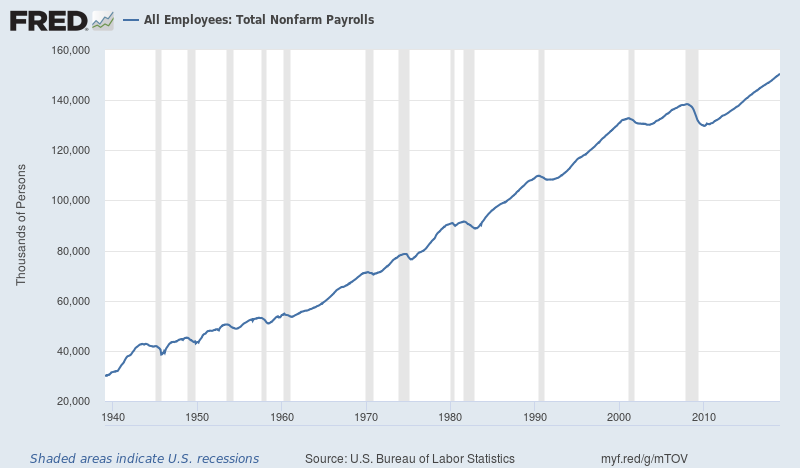
\includegraphics[width=5in]{./resources/nonfarm_level.png}
\end{center}
\end{frame}







\section*{Thanks!}

\end{document}